\documentclass[11pt,english,singlespacing,headsepline,consistentlayout]{auxiliary/si-msc-thesis}

\usepackage[utf8]{inputenc} % Required for inputting international characters
\usepackage[T1]{fontenc} % Output font encoding for international characters

\usepackage{float}
\usepackage{mathpazo}
\usepackage{setspace}
\usepackage{listings}
\usepackage{caption}
\usepackage{subcaption}
\usepackage[ruled]{algorithm2e}

\setlength\parindent{0pt}

%%%%%%%%%%%%%%%%%%%%%%%%%%%%%%%%%%%%%%%%%%%%%%%%%%%%%%%%%%%%%%%%%
%%%	MARGIN SETTINGS %%%%%%%%%%%%%%%%%%%%%%%%%%%%%%%%%%%%%%%%%%%%%
%%%%%%%%%%%%%%%%%%%%%%%%%%%%%%%%%%%%%%%%%%%%%%%%%%%%%%%%%%%%%%%%%

\geometry{paper=a4paper, inner=1.5cm, outer=1.5cm, bindingoffset=0cm, top=1.5cm, bottom=1.5cm, footnotesep=1cm, 
	%showframe, % Uncomment to show how the type block is set on the page
}

%%%%%%%%%%%%%%%%%%%%%%%%%%%%%%%%%%%%%%%%%%%%%%%%%%%%%%%%%%%%%%%%%
%%%	THESIS INFORMATION %%%%%%%%%%%%%%%%%%%%%%%%%%%%%%%%%%%%%%%%%%
%%%%%%%%%%%%%%%%%%%%%%%%%%%%%%%%%%%%%%%%%%%%%%%%%%%%%%%%%%%%%%%%%


\thesistitle{Instrumentation and\\
Performance Analysis\\of Distributed Systems\\ with Freud}



%comment to not have subtitle
%\thesissubtitle{} 

\author{Stefano Taillefert}

\monthyear{May 2021}

\supervisor{Prof. Antonio Carzaniga}

% if you need to add or remove co-supervisors go into titlepage.tex and comment correspondingly

\cosupervisorone{None}
\cosupervisortwo{None}
\cosupervisorthree{None}

%%%%%%%%%%%%%%%%%%%%%%%%%%%%%%%%%%%%%%%%%%%%%%%%%%%%%%%%%%%%%%%%%
%%%	FRONT MATTER %%%%%%%%%%%%%%%%%%%%%%%%%%%%%%%%%%%%%%%%%%%%%%%%
%%%%%%%%%%%%%%%%%%%%%%%%%%%%%%%%%%%%%%%%%%%%%%%%%%%%%%%%%%%%%%%%%

\begin{document}

\frontmatter
\pagestyle{plain}

%%%%%%%%%%%%%%%%%%%%%%%%%%%%%%%%%%%%%%%%%%%%%%%%%%%%%%%%%%%%%%%%%
%%%	TITLE PAGE %%%%%%%%%%%%%%%%%%%%%%%%%%%%%%%%%%%%%%%%%%%%%%%%%%
%%%%%%%%%%%%%%%%%%%%%%%%%%%%%%%%%%%%%%%%%%%%%%%%%%%%%%%%%%%%%%%%%

%%%%%%%%%%%%%%%%%%%%%%%%%%%%%%%%%%%%%%%%%%%%%%%%%%%%%%%%%%%%%%%%%
%%%	TITLE PAGE %%%%%%%%%%%%%%%%%%%%%%%%%%%%%%%%%%%%%%%%%%%%%%%%%%
%%%%%%%%%%%%%%%%%%%%%%%%%%%%%%%%%%%%%%%%%%%%%%%%%%%%%%%%%%%%%%%%%

\begin{titlepage}

\hspace{-11.8mm} 
\includegraphics[width=65mm]{auxiliary/usi-inf-logo.png}

\linespread{1.25}
\vspace{24mm} \hspace{26mm} \parbox{127mm}{{\bf {\huge {\ttitle}}\par}}
\linespread{1}

\ifthenelse{\boolean{@subtitle}}
	{\vspace{4mm} \hspace{26mm} \parbox{127mm}{{\bf {\large {\em {\subtitle}}}}}\vspace{10mm}}
	{\vspace{26.5mm}}

\vspace{16mm} \hspace{26mm} \parbox{127mm}{{\Large {\textbf{\authorname}}}}

\vspace{24mm} \hspace{26mm} {\large \moyear}

\vspace{48mm} \hfill {\large {\em Supervised by}}\\ \vspace{1mm} \hfill {\large {\bf {\supname}}}

%\vspace{8mm} \hfill {\large {\em Co-Supervised by}}\\ \vspace{1mm} \hfill {\large {\bf {\cosupnameone}}}

%comment out if it does not apply

%\vspace{1mm} \hfill {\large {\bf {\cosupnametwo}}}

%\vspace{1mm} \hfill {\large {\bf {\cosupnamethree}}}


\vfill

\hfill \noindent {\textsc{Bachelor Project}}

\end{titlepage}

%%%%%%%%%%%%%%%%%%%%%%%%%%%%%%%%%%%%%%%%%%%%%%%%%%%%%%%%%%%%%%%%%
%%%	ABSTRACT %%%%%%%%%%%%%%%%%%%%%%%%%%%%%%%%%%%%%%%%%%%%%%%%%%%%
%%%%%%%%%%%%%%%%%%%%%%%%%%%%%%%%%%%%%%%%%%%%%%%%%%%%%%%%%%%%%%%%%

\begin{abstract}
  Engineering software systems for performance is a particularly
  complex task.  The performance of a software system depends on many
  factors, such as the algorithmic nature of the software, the
  features of the execution environment (including memory, storage,
  and CPU) and the complex interactions between components, whether
  internal or external.  A common way to support performance analysis
  is to create models of the system.  This can be done, for example,
  with traditional profilers, which characterize the distribution of
  the CPU time expenditures on functions and methods.

  Freud is a software performance analysis tool that derives similar
  but more expressive models called performance annotations.  In
  essence, such annotations characterize a relevant performance metric
  (e.g. CPU time) as a function of one or more input parameters or
  features.  In particular, Freud derives performance annotations
  automatically based on measurements of a software system.  The goal
  of this project, called \emph{Jung}, is to extend Freud to
  instrument and collect data from \emph{distributed} systems. This
  means augmenting the existing implementation to instrument and
  collect performance metrics from a number of distributed components.
  Jung applies this instrumentation and collects data through a
  communication framework, and subsequently links and merges
  independent component traces using causal relations.  The resulting
  unified trace is then fed into the Freud statistical analyzer to
  produce meaningful annotations.

  Jung can therefore be used to support the performance engineering
  of applications that use and connect to external
  resources, such as databases and other services.
\end{abstract}


%%%%%%%%%%%%%%%%%%%%%%%%%%%%%%%%%%%%%%%%%%%%%%%%%%%%%%%%%%%%%%%%%
%%%	DEDICATION & ACKNOWLEDGEMENTS %%%%%%%%%%%%%%%%%%%%%%%%%%%%%%%
%%%%%%%%%%%%%%%%%%%%%%%%%%%%%%%%%%%%%%%%%%%%%%%%%%%%%%%%%%%%%%%%%

%\dedicatory{Dedicated to whoever is reading this awesome piece of work}

\begin{acknowledgements}

\addchaptertocentry{\acknowledgementname}

The acknowledgments and the people to thank go here, don't forget to include your thesis advisor\ldots

\lipsum[1-6]

\end{acknowledgements}


%%%%%%%%%%%%%%%%%%%%%%%%%%%%%%%%%%%%%%%%%%%%%%%%%%%%%%%%%%%%%%%%%
%%%	PREAMBLE %%%%%%%%%%%%%%%%%%%%%%%%%%%%%%%%%%%%%%%%%%%%%%%%%%%%
%%%%%%%%%%%%%%%%%%%%%%%%%%%%%%%%%%%%%%%%%%%%%%%%%%%%%%%%%%%%%%%%%

\tableofcontents 
%\listoffigures 
%\listoftables

%%%%%%%%%%%%%%%%%%%%%%%%%%%%%%%%%%%%%%%%%%%%%%%%%%%%%%%%%%%%%%%%%
%%%	MAIN MATTER %%%%%%%%%%%%%%%%%%%%%%%%%%%%%%%%%%%%%%%%%%%%%%%%%
%%%%%%%%%%%%%%%%%%%%%%%%%%%%%%%%%%%%%%%%%%%%%%%%%%%%%%%%%%%%%%%%%

\mainmatter
 
\pagestyle{thesis} 

%\chapter{Introduction}

Bla bla intro stuff

\lipsum[1-20]

\chapter{Introduction}

Freud~\cite{freud} is a software performance analysis tool that
derives performance annotations from measurements of running
systems. What does that mean?  Freud requires the system in binary
form, although it can also benefit from the source code for additional
analysis.  In essence, Freud performs a dynamic analysis of the
system, meaning that it uses information derives from the execution of
the system under workloads chosen by the performance engineer.  Given
the program executable, compiled to include debugging symbols, Freud
instruments the system to measure a series of metrics, such as running
time and memory usage, while also tracing the function calls and their
parameters. Freud then analyzes this data (offline) to produce
significant statistical models that characterize the performance
metrics as functions of one or more input parameters (or
``features'').

The goal of this project is to extend Freud to collect and analyze
data from a \emph{distributed} software system.  This includes desktop
or server applications that might use external services, typically
through remote procedure calls (RPC), or a web application components
that query external servers such as a database.  To highlight the
relation with the Freud tool and technique, we decided to name this
project Jung --- after influential Swiss psychiatrist and psychoanalyst
Carl Jung\footnote{\url{https://en.wikipedia.org/wiki/Carl_Jung}} who
was a colleague and collaborator of Sigmund Freud.

In essence, Jung instruments a distributed system so that each
distributed component would measure various performance metrics of
interest.  The measurements are initially stored as separate traces
within each component.  Jung then takes care of collecting and merging
these separate traces so as to assemble a unified trace that would
then be processed through the statistics module of Freud.  In
particular, the instrumentation provided by Jung traces related calls
\emph{across} distributed components using unique identifiers.  The 
relation between calls amount to causal relations and therefore are
used as a basis for the merge operation.

Freud uses a powerful binary instrumentation framework called
Pin~\cite{PIN}.  In the initial prototype we developed during this
project, we opted for a simpler solution, and therefore decided to
inject our instrumentation directly within the source code, manually.
A fully automatic instrumentation could be added in future
developments to reduce the overhead of using Jung.


\chapter{Performance analysis}

% What is it, problem context, existing solutions in general

Performance engineering amounts to measuring, modeling, and ultimately
improving the performance of software systems.  Performance
engineering is crucial for many software systems.  For example, a
company such as Google that runs global-scale services and
applications is very concerned about performance.  The response time
of applications, such as GMail, can severely influence their adoption
and therefore their success or failure.  The same is definitely true
for web search and many other applications.  Even relatively minor
speed-ups or slow-downs can make a significant difference in usability
and therefore profitability.  In sum, performance engineering is
important.

Performance engineering is also difficult.  Many factors affect
performance in many often subtle ways.  There is the the algorithmic
complexity, but there are also other factors, including hardware
features and, crucially, the interactions between components within
applications, and across applications.  For example, a cache system
(memory or otherwise) can significantly improve the performance of a
system.  However, the mixed use of the same caching system by many
components or systems can drastically reduce its effectiveness
overall.

Performance analysis is primarily a type of dynamic analysis, and
therefore it is based on the measurement of running systems.  Almost
every kind of application can be instrumented to collect a variety of
performance metrics.  Consistently with the description of Freud, we
use the term \emph{metric} to denote the values of performance
indicators such as execution time (or ``wall clock'' time), actual CPU
time or cycles, memory usage, lock holding time, and many more.  These
metrics can be used in various ways and are chosen by the performance
engineer accordingly to the type of application and the type of
analysis.  For example, lock-holding time is not a very significant metric
for a single-threaded application, but it might be of crucial
importance for a highly parallel application such as most modern
client-side and server-side applications.

\begin{figure}[htb]
  \centering
  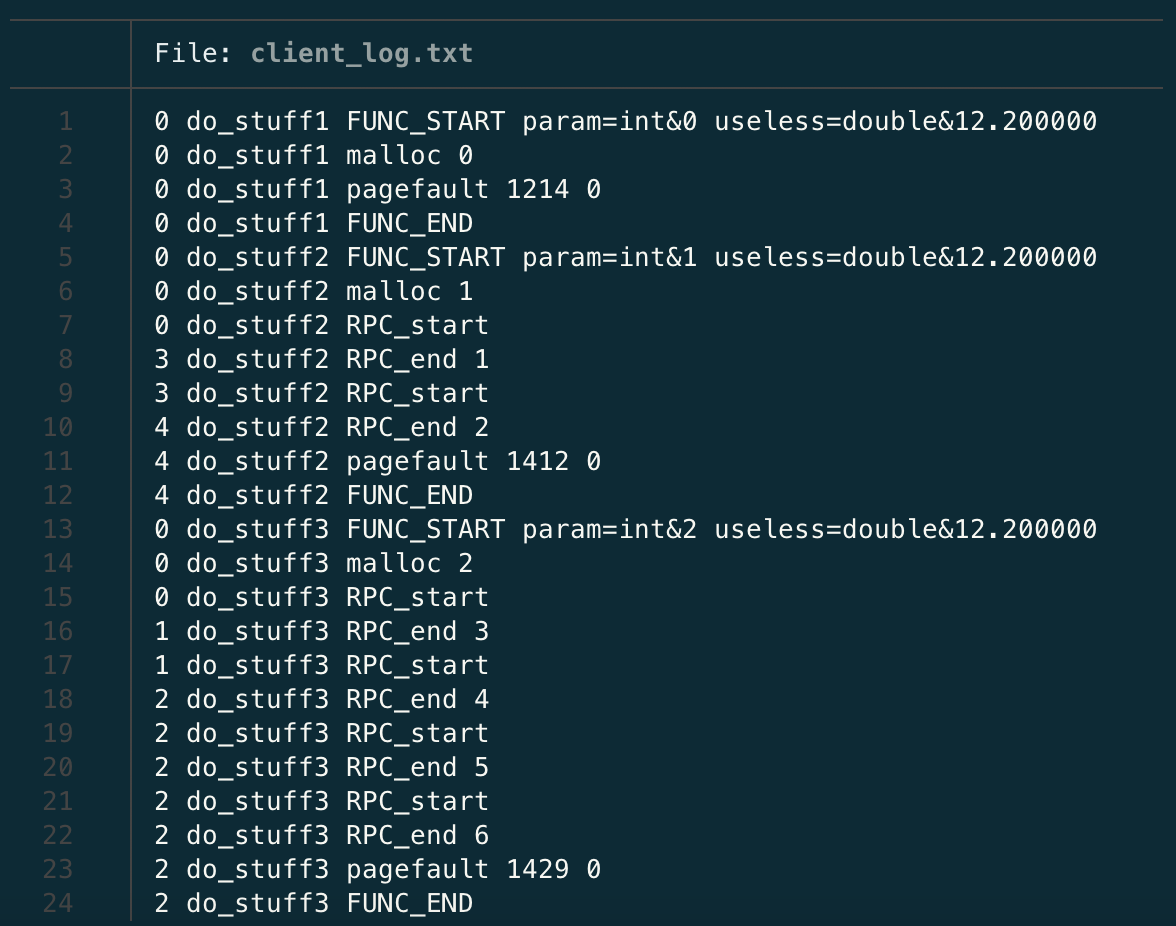
\includegraphics[width=0.65\textwidth]{clientLog.png}
  \caption{An example of performance trace (in this case, produced by Jung)}
  \label{fig:clientLog}
\end{figure}
%
Performance analysis have several tools at their disposal to perform
instrumentation, measurement, and summary analysis. For example, there
are a lot of existing tools and solutions out there---one of which
will be discussed in section \ref{sec:freud}---that can
\emph{instrument} the executables: a dedicated tool injects some
special code directly in the compiled binary file, following some
particular compiler flags. This generated code then measures different
parameters, keeping track for example of starting and ending times,
memory allocations, and so on.  At the end, an information dump is
produced to summarize the data, which can then be analyzed in various
ways.

In this project we focus on a specific problem and context, namely the
collection and combination of measurement traces for the analysis of
distributed systems.


\chapter{Project design}

\section{Freud}\label{sec:freud}

% Brief description, intro to Freud and PIN, what they do and how

This project follows the steps of Freud, a tool developed by Daniele
Rogora, an USI PhD student.  This software has multiple components;
the first two (\texttt{freud-dwarf} and \texttt{freud-pin}) are tasked
with instrumenting the executable via a special tool called PIN
\cite{PIN}, developed by Intel. This library---as explained earlier
---inserts the instructions necessary to collect the data during the
execution. Basically, coding this part means writing code that will
write some code to put into other code.

The other part of Freud, which is the one we will be interacting with, is \texttt{freud-statistics}.
As the name implies, this module (based on the popular \texttt{R} library\footnote{\url{https://www.r-project.org/}})
processes the statistics, resulting in a regression or clustering, given the output of the instrumentation.


\section{Requirements and analysis}\label{sec:requirements}

% Goals, what we needed to implement, refer to the plan and list of tasks, what's the idea

The main idea was to start small and build features incrementally, to
ensure that we always had a minimal working prototype.  The main
objective of Jung is to instrument multiple systems, collect the data
and format it.  To achieve this, we divided the project in three main
components:

\begin{itemize}
\item The actual instrumentation library, with an API to track the
various metrics
\item The merger, which has to collect all the log files from the
different systems and merge them in a single coherent trace
\item The dumper, which is tasked with creating the binary output that
will be passed to \texttt{freud-statistics}
\end{itemize}

The main milestones of the developments were the following: first we
had to develop a simple distributed application, based on an RPC
library, to be used as an initial test environment.  For this part we
chose to put together a relatively simple program that sends back and
forward some text messages; the server has some delays set up in
answering some queries to simulate a long computation.

Following that, we needed to develop an instrumentation for the client
side, server side, and --- crucially --- the RPC library: the idea was
to measure some meaningful statistics on all sides involved.  The
metrics we settled with are:

\begin{itemize}
            \item Execution time
            \item Memory usage
            \item Major and minor page faults
            \item Lock holding and waiting time
            \item Possible memory leaks (experimental)
        \end{itemize}

        The execution time is computed and accounted for separately
between client (total, end-to-end, synchronous), server, and network.
All other metrics are computed and accounted for the client and server
side.  All the chosen metrics except for the memory leak estimate are
supported by \texttt{freud-statistics}.  Possible memory leaks are
detected by tracing and matching the amount of \texttt{malloc} and
\texttt{free} calls.  However, this computation can only offer an
approximate leak detector.

        Then, we had to devise a method to save and retrieve the
measurement logs from all the components.  This has been done by
dumping the collected information in a text file with some special
encoding (see section \ref{sec:issues} for details) for data types and
more complex values.

        The next step was to design an algorithm to merge the logs
from all the systems into a single coherent trace. This was tricky
because we had to correctly identify all the remote calls to allow to
trace back which server execution corresponded to which client
function. We don't want to debit someone with the computing costs of
someone else, therefore we assigned unique IDs to each RPC call to
allow to trace back which client function requested which server
resource.

        Integrating said trace in the existing statistics tool
(\texttt{freud-statistics}) to derive the performance annotations was
the last objective for the coding part. For this we had to rely on the
help of its creator, Daniele, to fully understand how to format the
data. There were a few hiccups due to some technical issues, but the
process concluded perfectly.

        Unfortunately, the only abandoned part of the project was to
identify some third-party non-trivial distributed applications and
analyze them with the created tool. Due to the fact that Jung doesn't
work on the binary executable, we needed to access the source code of
the application we wanted to analyze. This heavily reduced the
spectrum of possible targets, and also considering the little time
left we decided to abandon it.

        Last but not least, we had to write the report, prepare the
poster and the presentation. Due to the current situation, we as a
class decided to not hold any presentation this year, therefore this
point got reduced to the document you're currently reading.
        
        Have a pizza: this is still on hold but will definitely be
completed sooner or later. Every project needs a celebratory pizza at
the end.
        

\chapter{Implementation}

    \begin{figure}[H] \centering
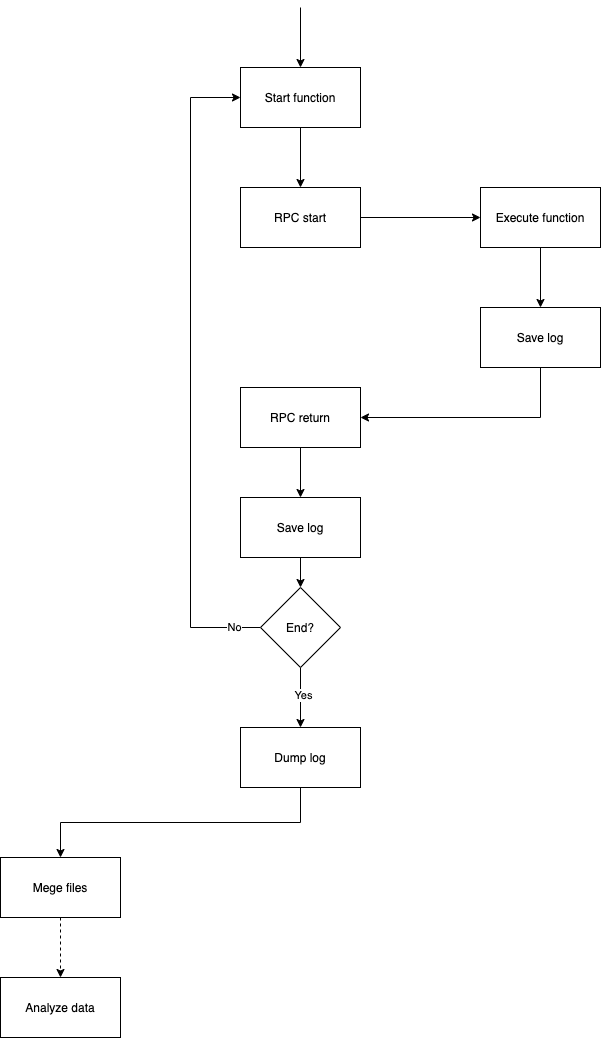
\includegraphics[width=0.6\textwidth]{schema.png}
        \caption{Jung's general functioning scheme}
        \label{fig:schema}
    \end{figure}
    

    \section{Technologies and tools used}

        We used gRPC \cite{gRPCdocs} as the RPC library, since it
seemed pretty straightforward and simple to use. There are plenty of
examples in the documentation and a lot of languages are supported,
including C++. On the other hand, Jung is independent from any
library: its functions can be used directly from the code, even in a
custom RPC implementation.

        The choice of language was pretty easy as well: Freud is built
entirely in C/C++, so using the same language would increase
compatibility. The only choice we had to make was regarding the
version: we went with C++17 to benefit from the
\texttt{filesystem::exists()} function, which we used to check for the
existence of previous log files.

        To simplify development and testing, we also packaged an
auto-building Docker image
(\url{https://hub.docker.com/repository/docker/steeven9/jung}) with
the example server in it.  This way we could keep the server running
on another machine and, for example, test the network times from
another remote location.


    \section{Issues}\label{sec:issues}

        The only major problem we had - which we believe to be very
common - was that we made some design choices in order to initially
simplify the job, but then, with the addition of new features or to
fix certain problems, we had to change approach. The direct
consequence was that we had to rewrite some large parts of the code
and data structures to adapt to the new requirements.
        
        One instance of the aforementioned problem is that we had to
develop some particular encoding to represent the function
parameters, since we had to convert from data (the running code) to
text (the log file) and vice versa. More specifically, we chose to
represent the values as \texttt{name\=type\&value}
(e.g. \texttt{asd\=int\&12} for an integer named \texttt{asd} of value
12); this added a supplementary layer of encoding/decoding when saving
and reading the data to/from the text files.

        When we first started testing the integration with
\texttt{freud-statistics}, since we was unable to see what was in the
binary file, we had troubles checking if we was dumping the metrics
correctly, resulting in some weird-looking statistics. With Daniele's
help, we managed to make sense of the output and find the offending
code parts to patch.

        And of course, we had our fair share of miscellaneous issues
with pointers, segmentation faults and general weird behaviors. As a
positive note, in the process we somehow created a program that frees
memory as you run it:

        \begin{figure}[H] \centering 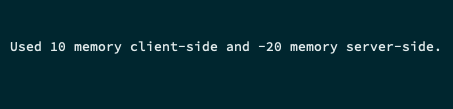
\includegraphics{memUsage.png}
            \caption{A very peculiar memory usage}
            \label{fig:memUsage}
        \end{figure}

        Another problem we ran into was that initially we were unable
to get \texttt{freud-statistics} to find a regression, despite our
data was clearly a good candidate for it. Turns out we simply didn't
have a good enough p-value, which was easily fixed by getting more
samples (details will follow in the next chapter).


\chapter{Evaluation}

    % Code validation, analysis of results and practical applications,
personal experience (?)

    Referring to the task list in section \ref{sec:requirements}, we
can assert that we successfully implemented all the required
features. The results the library provides are accurate (to a certain
extent) and repeatable.

    To test Jung's functionality we created a demo program that
simulates a real use-case of this library: a client program
(\texttt{jung\_client}) sends some requests to a server (you guessed
it, \texttt{jung\_server}) which computes the results and sends them
back. To make it more realistic, the server takes roughly the time in
seconds equal to the parameter received (with some added random
margin), since it simulates a computation. Being a single-threaded
sever, this has been achieved by making the server thread sleep for
the given input. On the other hand, the client uses a \texttt{for}
loop to send the requests, so the parameter's value increases
gradually; the maximum number of iterations has been set to 20 and the
number of points to 5, but those can easily be changed in the code
(\texttt{NUM\_MSG} and \texttt{NUM\_POINTS} respectively).

    Alas, time and coding constraints limited the amount of testing we
could do, meaning that the performance analysis has been tested only
with a few scenarios. The first one is illustrated in the plot below:

\begin{figure}[H] \centering
  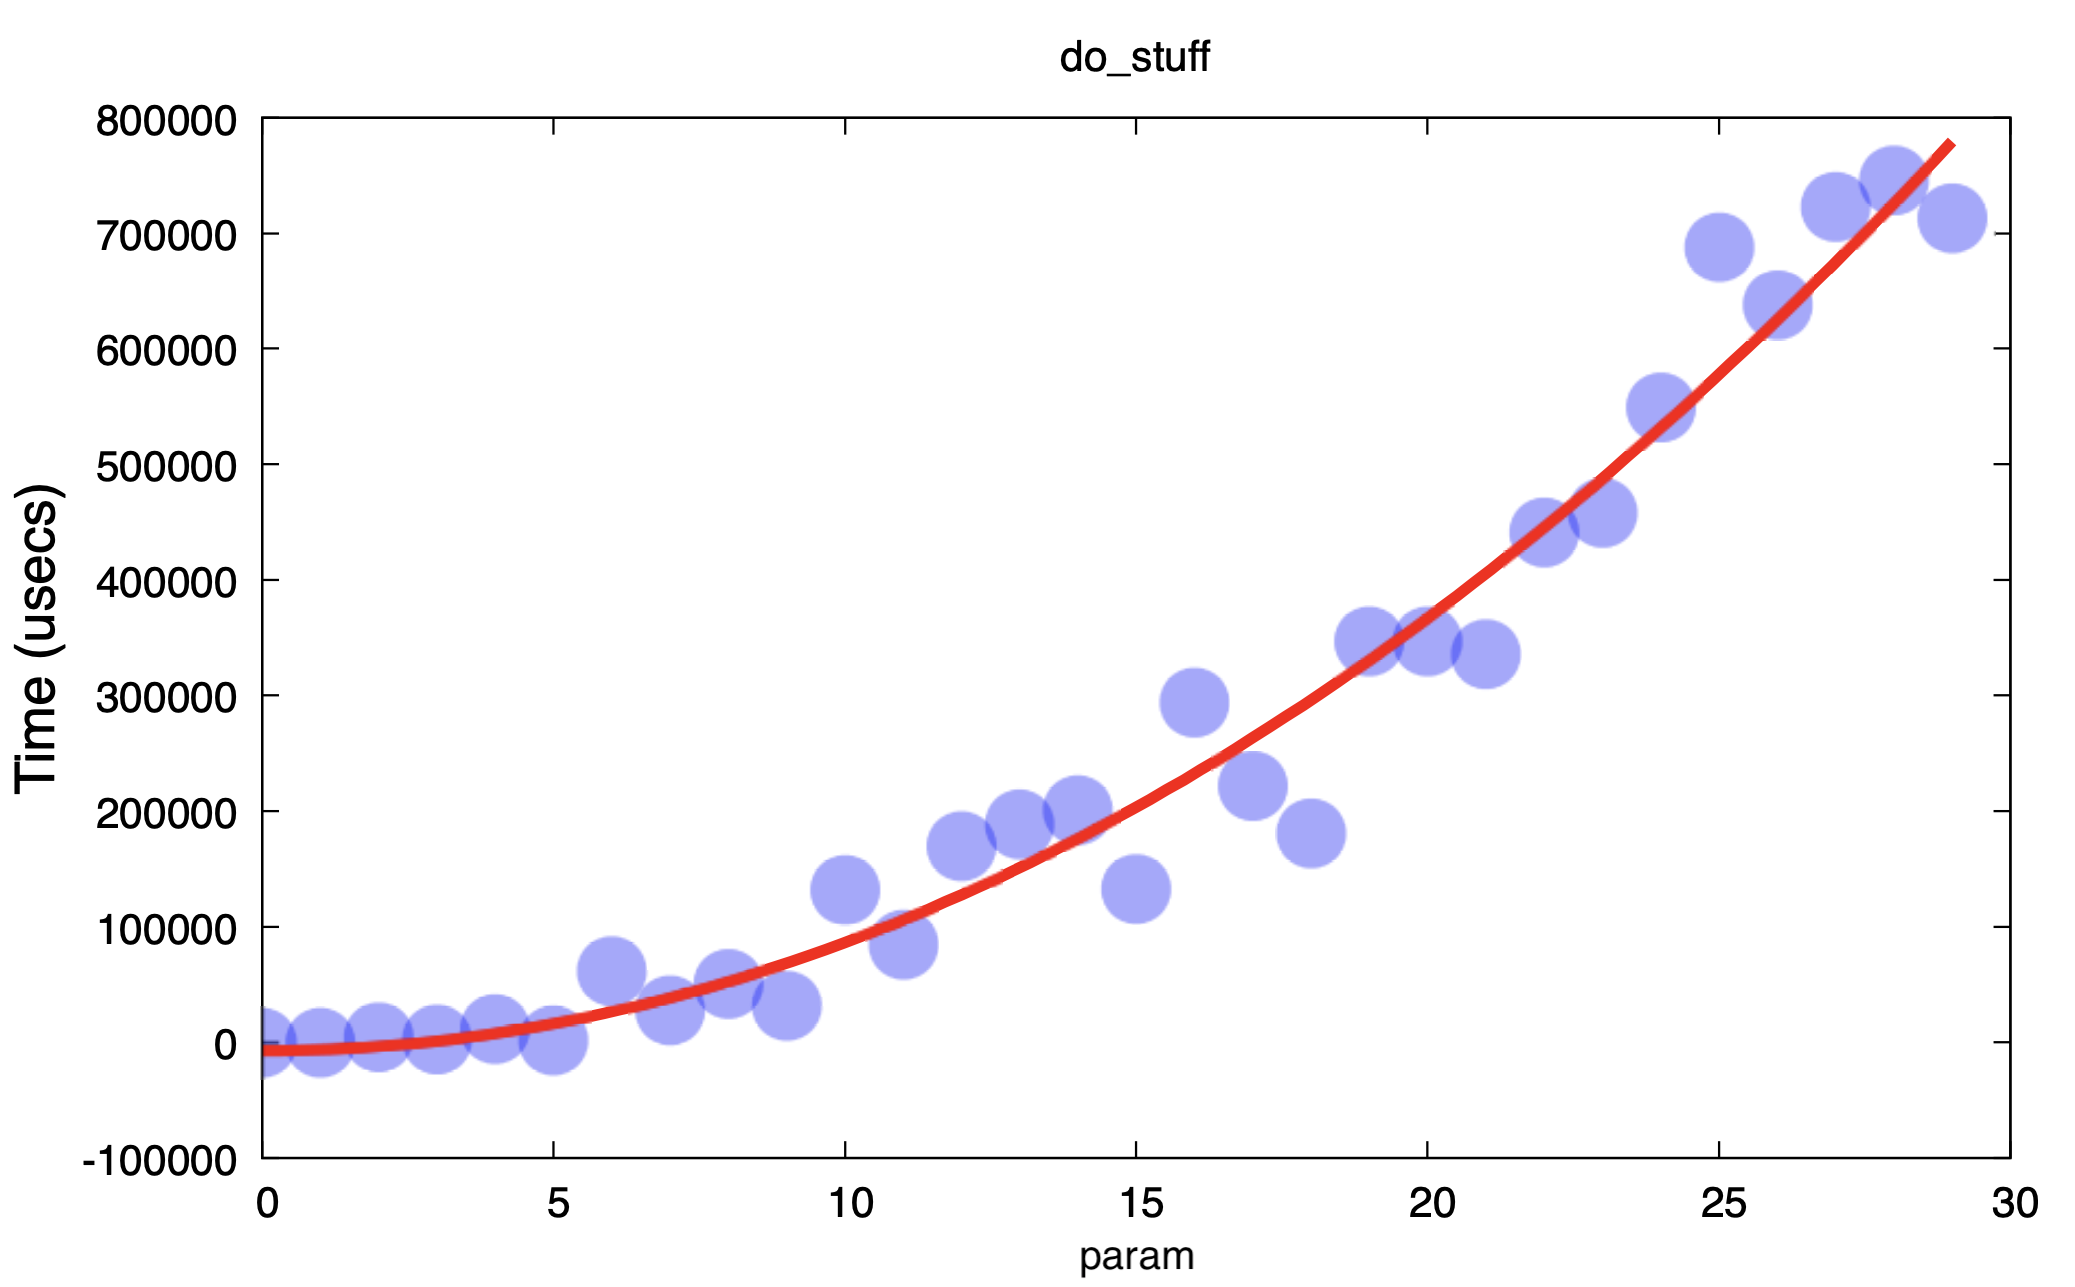
\includegraphics[width=0.7\textwidth]{analysis.png}
  \caption{The first plot produced by \texttt{freud-statistics}}
  \label{fig:analysis1}
\end{figure}

As we can see, our data fits nicely in a quadratic regression, as
expected; our client program can be represented with the following
algorithm:

\begin{algorithm}[H] \For{$i \gets 0$ \textbf{to} NUM\_MSG} {
    \For{$j \gets 0$ \textbf{to} NUM\_POINTS} { \For{$k \gets 0$
        \textbf{to} $i$} { sleep($k + $ random\_margin())\; } } }
  \caption{Quadratic simulation algorithm}
\end{algorithm}

\vspace{5mm}

Another scenario can be simulated by making the RPC calls a constant
amount of times instead of depending on the parameter, which produces
the linear result in the plot below:

\begin{figure}[H] \centering
  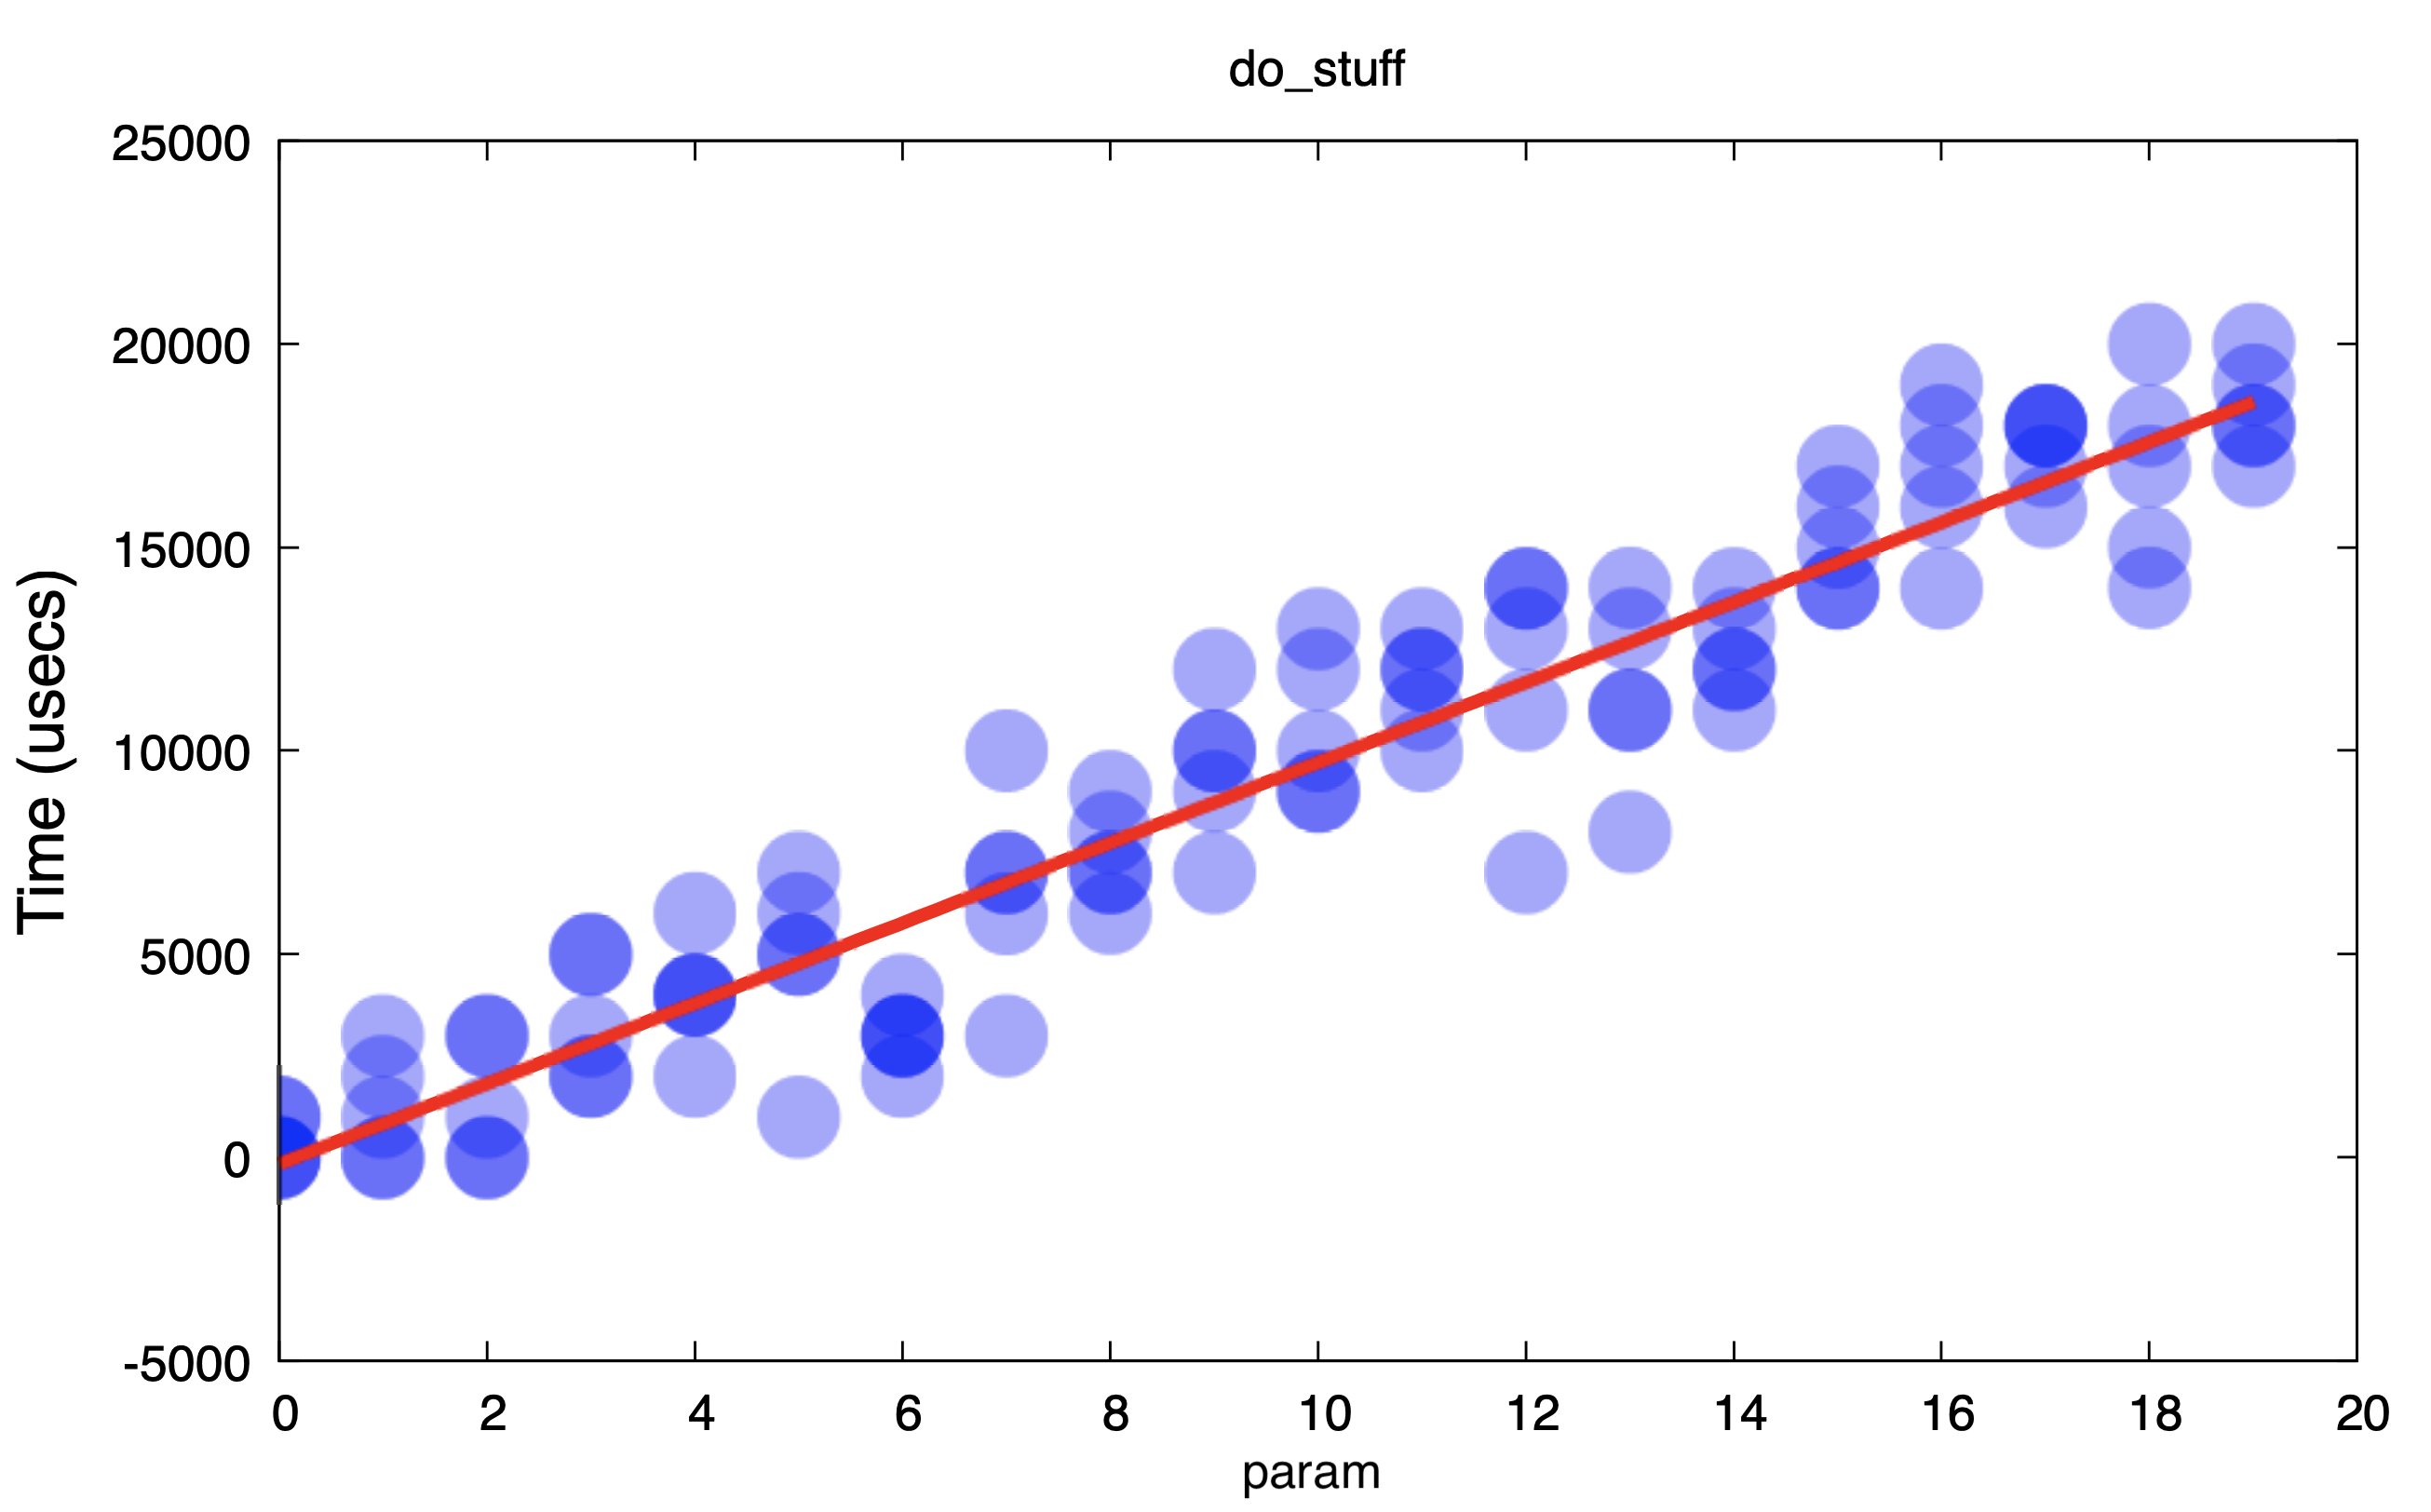
\includegraphics[width=0.7\textwidth]{analysis2.png}
  \caption{The second plot produced by
    \texttt{freud-statistics}}
  \label{fig:analysis2}
\end{figure}

And the corresponding elementary algorithm:

\begin{algorithm}[H] \SetAlgoLined \For{$i \gets 0$ \textbf{to}
    NUM\_MSG} { \For{$j \gets 0$ \textbf{to} NUM\_POINTS} { sleep($i + $
      random\_margin())\; } }
  \caption{Linear simulation algorithm}
\end{algorithm}

\vspace{5mm}


\section{Testing}

Due to the complexity and particular nature of the software,
we decided to not implement any automated tests. Opposed to
test-driven development, we had a more unstructured way of iterating
over the code, since the functionality had to be checked by hand by
comparing the produced log files with the program.  Therefore, the
effective coverage is 0\%, but as someone once said:

\begin{quote} \centering \textit{"Tests don't prove
    correctness"}
\end{quote}


\section{Demo}

In this section you can find instruction on how to run a demo
program and analyze the obtained data.

To install and compile all the required software, simply run the
\texttt{install.sh} script from the Jung repository.  In case of
failure, please refer to the READMEs of each project for more
information.

First, start the server:

\texttt{\$ ./jung\_server}

While in another shell, run the client:

\texttt{\$ ./jung\_client}

\textit{Note: if you run the server on another machine, you
  can pass the \texttt{---target=HOSTNAME} % three dashes in the
  sentence above render correctly dunno why leave it like that argument
  to the client.}

Then, with both the client and server log files in the root
folder, merge the traces:

\texttt{\$ ./trace\_merge}

This will produce the binary data (under \texttt{symbols/})
and a summary of the execution (\texttt{trace\_log.txt}).  We can then
run Freud's analysis tool:

\texttt{\$ cd ../freud/freud-statistics}

\texttt{\$ ./freud\_statistics 3 0 0 do\_stuff
  ../../Jung/symbols/do\_stuff/}

\textit{Note: this is an example, refer to Freud's
  documentation for details and usage.}

This should find a nice regression and plot it. That's it!


\chapter{Conclusions}

% Results wrt objectives, limitations

We consider the obtained results pretty satisfying: we managed to
realize a working application that complies with the requirements and
could be used in the field to measure actual systems (with some
limitations, of course). As the evaluation shows, Jung correctly
tracks and aggregates metrics, producing an output which can be
interpreted by another tool. Different behaviors are correctly picked
up and produce different outputs when analyzed, as expected.

From a more personal point of view, the whole project was a great
learning experience, both in terms of development and project
management; in addition to refreshing my C++ skills, I experienced
carrying out a large-ish project on my own, with deadlines and
constraints.  I would like to add that the way my advisor and I
organized the work was very helpful: small steps and weekly meetings
allowed to iterate quickly over the code and to keep relatively on
track with the schedule. As a matter of fact, the only discarded
feature, testing on third-party applications, was not mandatory for
the completion of the project.

\subsection*{Acknowledgements}

I'd like to thank Antonio, my advisor, for the opportunity and for
guiding me throughout this project; Daniele, Freud's author, for his
help understanding his amazing software; my friends Sasha and Brites
for their incredible support; and last but not least everyone that
supported me during these tiring times.

Thank you!


\section{Future work and possible developments}

While this project can be considered a success, there are
still a number of improvements that could be implemented. For example
a better handling of the data dumping via a separate thread: as of now
every function writes the buffered metrics to the log file when it
finishes executing. While this is barely noticeable on a small scale,
it could add a significant overhead under large loads or in
performance-critical systems.

A crucial missing part is an actual instrumentation like
Freud's, either through PIN or another similar library, allowing the
user to work on the executables instead of having to change the source
code.

Other possible improvements would be to support more complex
features as parameters, like structs, automatically infer the type of
the parameter (opposed as having to manually specify it), and export
the data in a more universal format, like csv, to be able to use it in
a wider variety of analysis tools.


%\appendix

%\chapter{Additional Things}

Appendix stuff

\lipsum[1-20]

%%%%%%%%%%%%%%%%%%%%%%%%%%%%%%%%%%%%%%%%%%%%%%%%%%%%%%%%%%%%%%%%%
%%% BIBLIOGRAPHY %%%%%%%%%%%%%%%%%%%%%%%%%%%%%%%%%%%%%%%%%%%%%%%%
%%%%%%%%%%%%%%%%%%%%%%%%%%%%%%%%%%%%%%%%%%%%%%%%%%%%%%%%%%%%%%%%%

\newpage \bibliographystyle{abbrv} \bibliography{biblio}

\end{document}